\documentclass{beamer}
\usetheme{CambridgeUS}
\usecolortheme{beaver}
\setbeamertemplate{navigation symbols}{}

\usepackage{amsmath}   % MUST come before \DeclareMathOperator
\usepackage{amssymb}
\usepackage{tikz}
\usepackage{tikz-3dplot}
\usepackage{pgfplots}
\usetikzlibrary{calc}

\DeclareMathOperator{\diam}{diam}

\title{Self-Similarity and Fractals}
% Short author for footline:
\author[Alex Cristaudo]{%
  Alex Cristaudo\\[6pt]
  \small\textit{Supervisor: Dr. Francois Ebobisse}
}

\institute{University of Cape Town}

\date{7 October 2025}

\begin{document}

%------------------------------------------------
\begin{frame}
  \titlepage
\end{frame}

%------------------------------------------------
\begin{frame}{Overview}
\tableofcontents
\end{frame}

%------------------------------------------------
\section{Introduction and Motivation}
\begin{frame}{Motivation and Context}
\begin{itemize}
    \item Fractals: infinitely complex objects, generally defined by simple rules. Most fractals we will look at are ``self-similar'' (i.e., made up of smaller parts of itself).
        \item Mandelbrot (1975): coined the term "fractal" as a shape whose Hausdorff dimension exceeds topological dimension.
    \item Applications: coastlines, clouds, mountains, finance, physics, economics.
    \item Aim of thesis: use self-similarity to investigate fractal properties via Hausdorff metric \& measure.
\end{itemize}
\end{frame}

%------------------------------------------------
\begin{frame}{Mathematical Tools}
The mathematical tools we need to investigate this are:
\begin{itemize}
    \item \textbf{Hausdorff Metric}: compares compact sets and allows us to talk about convergence of sets.
    \item \textbf{Hausdorff Measure \& Dimension}: a generalisation of Lebesgue measure to arbitrary metric spaces. Allows us to assign sizes to sets.
    \item \textbf{Self-Similarity}: allows us to explore how a fractal is defined geometrically
    \item \textbf{Open Set Condition (OSC)}: the connecting piece between self-similarity and the Hausdorff Measure, ensures minimal overlap of components of the fractal
\end{itemize}
\end{frame}

%------------------------------------------------
\section{The Hausdorff Metric}
\begin{frame}{The Hausdorff Metric}
Let $(X,d)$ be a metric space and let $A, B \subseteq X$, $A \neq \emptyset$ and $x \in X$. Recall:
\[
d(x,A):=\inf_{a\in A} d(x,a),\qquad
d(A,B):=\sup_{a\in A} d(a,B)=\sup_{a\in A}\inf_{b\in B} d(a,b).
\]

\centering
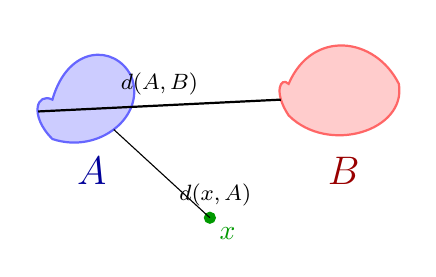
\begin{tikzpicture}[scale=1]
  \fill[blue!20, draw=blue!60, thick]
    (0,0) 
    .. controls (0.2,0.7) and (0.8,0.7) .. (1,0.3)
    .. controls (1.2,-0.2) and (0.6,-0.7) .. (0,-0.5)
    .. controls (-0.3,-0.2) and (-0.2,0.1) .. (0,0)
    -- cycle;
  \node[blue!60!black] at (0.5,-0.9) {\Large $A$};

  \fill[red!20, draw=red!60, thick]
    (3,0.2) 
    .. controls (3.3,0.9) and (4.1,0.8) .. (4.4,0.2)
    .. controls (4.5,-0.4) and (3.5,-0.7) .. (3,-0.2)
    .. controls (2.8,0.1) and (2.9,0.3) .. (3,0.2)
    -- cycle;
  \node[red!60!black] at (3.7,-0.9) {\Large $B$};

  \filldraw[green!60!black] (2,-1.5) circle (2pt) node[below right] {$x$};
  \coordinate (a_closest) at (0.78,-0.38);
  \draw (2,-1.5) -- (a_closest) node[midway, below right] {\footnotesize $\ d(x,A)$};
  \coordinate (a1) at (-0.18, -0.15);
  \coordinate (b1) at (2.9, 0);
  \draw[thick, black] (a1) -- (b1) node[midway, above] {\footnotesize $d(A,B)$};
\end{tikzpicture}
\end{frame}


\begin{frame}{Hausdorff metric (definition)}
Define
\[
\mathcal{K}(X)=\{A\subseteq X:\ A\ \text{is compact},\ A\neq\emptyset\}.
\]
Then
\[
d_H(A,B):=\max\{d(A,B),\,d(B,A)\}
\]
is a metric on $\mathcal{K}(X)$. This is called the induced Hausdorff metric with respect to the metric space $(X,d)$. Moreover $(\mathcal{K}(X),d_H)$ is complete iff $(X,d)$ is complete.
\end{frame}

%------------------------------------------------
\section{The Hausdorff Measure and Dimension}
\begin{frame}{Hausdorff measure (definition)}
Let $(X,d)$ be a metric space with $\diam(\emptyset):=0$. For $s\ge 0$, $\delta>0$ define
\[
\mathcal{H}^s_\delta(A)
:=\inf\Big\{\sum_{n=1}^\infty \big(\diam(E_n)\big)^s :\ A\subseteq\bigcup_{n=1}^\infty E_n,\ \diam(E_n)\le\delta\Big\}.
\]
If $A$ does not possess any $\delta$-coverings, we have $\mathcal{H}_\delta ^d(A) := \inf \emptyset =\infty $.
The Hausdorff $s$-measure is
\[
\mathcal{H}^s(A):=\lim_{\delta\to 0^+}\mathcal{H}^s_\delta(A)=\sup_{\delta>0}\mathcal{H}^s_\delta(A).
\]
If $ d=0$: Define $\diam (\emptyset)^0=0$ and use the interpretation $0^0=1$ for any other sets.
\end{frame}

%------------------------------------------------
\begin{frame}{Important properties}
\begin{itemize}
  \item It is an outer measure on $X$. So it is a measure on the $\sigma$-algebra of Hausdorff measurable sets
  \item In the Euclidean space, $(\mathbb{R}^n, d_E)$, the Hausdorff measure recovers Lebesgue measure (up to normalising constant) on for $n \in \mathbb{N}^+$. In any metric space, $\mathcal{H}^0$ is the counting measure. For $A \subseteq \mathbb{R}^n$,
  \[
  \lambda _n (A) = \frac{\pi ^{n/2}}{2^n \ \Gamma (n/2 + 1)} \mathcal{H}^n(A), \quad \Gamma (t):= \int \limits _0 ^\infty e^{-x}x^{t-1}dx 
  \]
  \item Invariant under isometries: If $f: X \to X$ is an isometry, then for any $A \subseteq X$, $\mathcal{H}^n(A) = \mathcal{H}^n(f(A))$
  \item Translation and scaling relationships: In metric space $(\mathbb{R}^n, d_E)$, $\mathcal{H}^n (A) = \mathcal{H}^n(A + \mathbf{x})$ and for $\lambda > 0$, $\mathcal{H}^n(\lambda A) = \lambda^n \mathcal{H}^n(A)$ 
\end{itemize}
\end{frame}

%------------------------------------------------

\begin{frame}{Important properties}
\begin{itemize}
\item Let $(X,d)$ be a metric space, $A \subseteq X$, and $0\le s<t$. Then $\mathcal{H}^s(A)<\infty\Rightarrow\mathcal{H}^t(A)=0$ and $\mathcal{H}^t(A)>0\Rightarrow\mathcal{H}^s(A)=\infty$.
  \begin{itemize}
  \item This creates a ``threshold behaviour" for any set $A$
  \item If $\mathcal{H}^d(A)$ is a finite, nonzero value, then for every $s \in [0,\infty)$ with $s \ne d$, we either have $\mathcal{H}^s(A)$ is infinite, or zero. More specifically, \begin{center}
    $\mathcal{H}^s(A) = \begin{cases}
        \infty  & \text { if }s < d \\ \text{finite, nonzero number} & \text { if } s = d \\ 0   & \text { if }s > d
    \end{cases}$
  \end{center}
  \item At this critical dimension, the measure value may be zero or infinite. Moreover, the dimension may be zero or infinite.
\end{itemize}
\end{itemize}
\end{frame}

\begin{frame}{The Hausdorff Dimension}
 Visually, the graph looks something like:
        \begin{center}

    \begin{tikzpicture}[font=\sffamily, scale = 0.5]
  % --- tweak this to move the critical exponent d ---
  \def\dval{2.0}
  \def\ymax{6.5}

  \begin{axis}[
    width=13cm, height=7.5cm,
    axis lines=middle,
    xlabel={$s$}, ylabel={$\mathcal{H}^s(A)$},
    xmin=-0.5, xmax=4.5, ymin=0, ymax=7.5,
    xtick={\dval}, xticklabels={$d$},
    ytick=\empty,
    clip=false,
    xlabel style={at={(axis description cs:0.98,0.02)},anchor=south east},
    ylabel style={rotate=90,anchor=south west},
    ]

    % LEFT: blow-up as s -> d^-
    % Use a reciprocal branch clipped at ymax for neatness
    \addplot [domain=0:{\dval-0.02}, samples=300, very thick, smooth, line cap=round, blue!70!black]
      {6.5};

    % RIGHT: decays to zero for s > d (use an exponential-like tail)
    \addplot [domain={\dval+0.02}:4.4, samples=300, very thick, smooth, blue!70!black]
      {0};

    % Vertical dashed line marking s = d (for clarity)
    \draw[dashed, gray!60] (axis cs:\dval,0) -- (axis cs:\dval,\ymax);

    % Finite marker at s = d (choose a modest finite value)
    \filldraw[black] (axis cs:\dval,3.15) circle (2.5pt);
    \node[right =5pt] at (axis cs:\dval,3.15) {$\mathcal{H}^d(A)\ \text{finite}$};

    % = infinity
    \node[right, align=left] at (axis cs:\dval + 0.1,6.5) {$= \infty$};

    % Open circles at turning points
    \filldraw[white] (axis cs:\dval,6.5) circle (2.5pt);
    \draw[line width=0.8pt] (axis cs:\dval,6.5) circle (2.5pt);

    \filldraw[white] (axis cs:\dval,0) circle (2.5pt);
    \draw[line width=0.8pt] (axis cs:\dval,0) circle (2.5pt);

    

    % Zero label + arrow on the right
    \node[right, align=left] at (axis cs:2.6,-0.45) {$\mathcal{H}^s(A)=0$ for $s>d$};


    % Region labels
    \node[left, align=center] at (axis cs:1.8,6.9) {$\mathcal{H}^s(A)=\infty$ for $s<d$};
  \end{axis}

\end{tikzpicture}

      \end{center}  
In this graph, we will say that the dimension of set $A$ is this critical point $d$. 
    For a set $A \subseteq X$, the Hausdorff dimension is a map $\dim_H : \mathcal{P}(X) \to [0,\infty]$ defined by:
        \begin{align*}
            \dim_H(A) := \inf\{d \geq 0 : \mathcal{H}^d(A) = 0\} = \sup\{d \geq 0 : \mathcal{H}^d(A) = \infty\}
        \end{align*}
        For this definition, we take $\sup \emptyset =0$ and $\inf \emptyset = \infty$
% At the critical dimension $d = \dim_H(A)$, we have $\mathcal{H}^d(A) \in [0, \infty ]$ and $\dim A \in [0,\infty ]$ (both need not be non-zero and finite) .

\end{frame}

%------------------------------------------------
\begin{frame}{Important Properties of the Hausdorff Dimension}
\begin{itemize}
    \item Let $(X,d_X)$ and $(Y, d_Y)$ be metric spaces. A map $f: X\to Y$ is bi-lipschitz if there is some real number $\alpha \ge 1$ such that \[\frac{1}{\alpha} d_X(x,y)\le d_Y(f(x), f(y))\le \alpha d_X(x,y)\]Let $f: X \to X$ be a bi-lipschitz map and $A \subseteq X$. Then $\dim _H(A) = \dim _H (f(A))$
    \item In metric space $(\mathbb{R}^n, d_E)$, $\dim_H (A + \mathbf{x}) = \dim _H(A)$ and $\dim_H (\lambda A) = \dim _H(A)$
    \item Monotonicity: If $A \subseteq B$, then $\dim _H A \le \dim _H B$
    \item Stable under countable unions: $\dim _H \left ( \bigcup \limits _{n=1}^{\infty} A_n \right) = \sup \limits _{n \in \mathbb{N}^+} \dim _H(A_n)$
    \item It agrees with our usual notion of dimensions: lines are 1-dimensional, squares are 2-dimensional, cubes are 3-dimensional while also assigning dimensions to irregular sets.
\end{itemize}
\end{frame}

%------------------------------------------------
\section{Self-Similarity}
\begin{frame}{Self-Similarity}
A map $S: \mathbb{R}^n \to \mathbb{R}^n$ is called a \textit{similitude} if there exists $r \in (0,1)$  such that \[
    |S(\mathbf{x}) - S(\mathbf{y})| = r |\mathbf{x}-\mathbf{y}|, \quad \text{ for all } \mathbf{x}, \mathbf{y} \in \mathbb{R}^n
    \]
    These are simply contractions in metric space $(\mathbb{R}^n, d_E)$. We call $r$ the contraction ratio of $S$.
    ~\\~\\An Iterated Function System (IFS) is a finite collection $\mathcal{S}=\{S_k:\mathbb{R}^n \to \mathbb{R}^n\}_{k=1}^N$ of similitudes with $N\ge 2$, and contraction ratios $r_1, ..., r_N$. 
    ~\\~\\A non-empty compact set $K$ is invariant under $\mathcal{S}$ if $K = \bigcup \limits _{k=1}^N S_k(K)$
\end{frame}

%------------------------------------------------
\begin{frame}{Self-Similarity Extended}
  \begin{itemize}
    \item For an Iterated Function System $\mathcal{S}$, there is a unique compact set invariant under $\mathcal{S}$
    \item Let $\mathcal{S}$ be an IFS. If \[
    \sum \limits_{i=1}^N r_i^D = 1
    \]then we call $D$ the \textit{similarity dimension} of $\mathcal{S}$ (denoted $\dim _S\mathcal{S} $).
    \item \textbf{OSC: The Open Set Condition}: An IFS $\mathcal{S}$ satisfies the \textit{Open Set Condition} if there exists a nonempty open set $O$ such that \[\bigcup \limits _{i=1}^N S_i(O) \subseteq O \text{ and } S_i(O) \cap S_j(O) = \emptyset \text{ for } i \ne j\]
  \end{itemize}
\end{frame}

\begin{frame}{Self-Similarity Final}
\begin{itemize}
  \item Let $K$ be the unique invariant set under $\mathcal{S} = \{S_i\}_{i=1}^N$, and $s = \dim _H K$. Then $K$ is self-similar if \[\mathcal{H}^s(S_i(K) \cap S_j(K)) = 0\] for $ i \ne j$ and $1\le i,j \le N$, $i,j \in \mathbb{N^+}$
  \item If $\mathcal{S}$ satisfies the OSC, then the invariant set $K$ of $\mathcal{S}$ is self-similar and $0 < \mathcal{H}^D(K)<\infty$ where $D$ is the unique number for which \[
    \sum \limits _{i=1}^N r_i^D = 1
    \]
    That is, $\dim _S \mathcal{S} = \dim _H K$ (the similarity dimension is the same as the Hausdorff dimension). This gives us an easy way to calculate the dimension of self-similar sets.
\end{itemize}
\end{frame}


%------------------------------------------------
\section{Classical Fractals}
\begin{frame}{The Cantor Set}
\begin{minipage}{0.6 \textwidth}
\small{
\begin{itemize}
        \item Begin with the interval $C_0 =[0,1]$
    \item Remove the middle third $(\frac{1}{3}, \frac{2}{3})$ to get $C_1 = [0, \frac{1}{3}] \cup [\frac{2}{3}, 1]$
    \item Remove the middle third from each remaining interval to get $C_2 = [0, \frac{1}{9}]\cup [\frac{2}{9}, \frac{1}{3}] \cup [\frac{2}{3}, \frac{7}{9}] \cup [\frac{8}{9}, 1]$
    \item Continue this process indefinitely, with $C_n$ the result at the $n$th iteration
    \item The Cantor set is the set as $n \to \infty$, that is, $\mathcal{C} := \lim _{n \to \infty}C_n= \bigcap \limits _{n\in \mathbb{N}_0}C_n$
    
\end{itemize}}
\end{minipage}%
\begin{minipage}{0.39 \textwidth}
  \begin{center}
\includegraphics[width = \textwidth]{assets/cantor.png}    
\end{center}
\end{minipage}
\end{frame}

\begin{frame}{The Cantor Set}
\begin{minipage}{0.6 \textwidth}
\small{
\begin{itemize}
  \item We can alternatively defined the Cantor set in terms of similitudes. Notice that if $C_0 = [0,1]$, then $C_{n+1} = \frac{C_{n}}{3} \cup (\frac{C_n}{3} + \frac{2}{3})$
  \item So for similitudes $S_1 (x) = \frac{1}{3}x$ and $S_2 (x) = \frac{1}{3}x + \frac{2}{3}$, we get that \[
  \mathcal{C} = S_1 (\mathcal{C}) \cup S_2(\mathcal{C})
  \]
  \item So the Cantor Set $\mathcal{C}$ is the unique invariant set under $\{S_1, S_2\}$.
  \item Thus finding $d := \dim _H \mathcal{C} = \dim _S \{S_1,S_2\}$ is the same as finding the solution to \[
  2\left ( \frac{1}{3} \right)^d = 1 \iff d = \frac{\ln 2}{\ln 3}
  \]
    
    
\end{itemize}}
\end{minipage}%
\begin{minipage}{0.39 \textwidth}
  \begin{center}
\includegraphics[width = \textwidth]{assets/cantor.png}    
\end{center}
\end{minipage}
\end{frame}

\begin{frame}{The Cantor Set Further Properties}
  \begin{itemize}
    \item It is totally disconnected
    \item It is uncountable
    \item It is a set with an irrational dimension $< 1$
    \item So $\lambda _1 (\mathcal{C}) = 0$
    \item It is self-similar and $\mathcal{H}^{\ln 2 / \ln 3} (\mathcal{C}) > 0$
  \end{itemize}
\end{frame}


\begin{frame}{The Koch Snowflake}
\begin{minipage}{0.6 \textwidth}
\small{
To geometrically construct the Koch Snowflake, start with an equilateral triangle (say of side length 1). Then recursively, for each line segment,
\begin{itemize}
    \item Divide the line segment into 3 segments of equal length
    \item Draw an equilateral triangle that has the middle segment as its base and points outward
    \item Remove the line segment that is the base of this triangle
\end{itemize}
}
\end{minipage}%
\begin{minipage}{0.39 \textwidth}
  \begin{center}
\includegraphics[width = \textwidth]{assets/koch_snowflake.png}    
\end{center}
\end{minipage}
~\\~\\
\begin{itemize}
\item We can show that the Hausdorff dimension is $\frac{\ln 4}{\ln 3}$
\item This is greater than 1 so the total length of the snowflake is $\infty$
\item We can show that the area inside the Koch Snowflake is $\frac{2 \sqrt{3}}{5}$
\end{itemize}

\end{frame}




\begin{frame}{Sierpiński Triangle \& Carpet}

\begin{minipage}{0.6 \textwidth}
\small{

The Sierpinski Triangle: 
\begin{itemize}
\item Start with an equilateral triangle (with its area, say side length 1).
\item Subdivide the triangle into 4 congruent triangles, and remove the middle triangle.
\item Repeat this recursively on all remaining triangles
\end{itemize}
~\\
The Sierpinski Carpet:
\begin{itemize}
\item Begin with a square (let's say $[0,1] \times [0,1]$).
\item Subdivide this square into 9 congruent squares, and remove the middle square.
\item Repeat this recursively on all remaining squares
\end{itemize}
}
\end{minipage}%
\begin{minipage}{0.39 \textwidth}

  \includegraphics[scale = 0.23]{assets/sierpinski_triangle.png}
  ~\\~\\~\\
  \includegraphics[scale = 0.2]{assets/sierpinski_carpet.png}
  
\end{minipage}
\end{frame}

\begin{frame}{Sierpiński Triangle \& Carpet properties}

\begin{itemize}
    \item Triangle dimension: $\displaystyle \frac{\ln 3}{\ln 2}\approx 1.585$.
    \item The triangle has infinite perimeter but no area
    \item Carpet dimension: $\displaystyle \frac{\ln 8}{\ln 3}\approx 1.893$.
    \item The carpet again has no area
\end{itemize}

\end{frame}

\begin{frame}{Pythagoras Tree}
  \small{
  Some fractals cannot use similitudes to describe. Instead we use the Hausdorff measure directly

\begin{itemize}
    \item Begin with a unit square (let's say the bottom left corner is (0,0)).
    \item On the top edge of this square, construct an 
    isosceles right triangle with the top edge as its hypotenuse. On each of the two equal sides of the triangle, construct a new square outward. 
    \item Repeat the process recursively on every new square. 

    \item We let $\mathcal{P}_n$ be the $n$-th iteration and the Pythagoras' Tree be $\mathcal{P}= \bigcup \limits _{n \in \mathbb{N}_0} \mathcal{P}_n$
    
\end{itemize}
\begin{center}
        \includegraphics[scale = 0.3]{assets/p_tree_one.png}
    \end{center}
  }
  We are bounded by how far the square extends outwards, and the tree contains the unit square so $0 < \mathcal{H}^2(\mathcal{P}) < \infty$. Thus $\dim _H \mathcal{P} = 2$
~\\
\end{frame}



%------------------------------------------------
\section{Conclusion}
\begin{frame}{Conclusion}
\begin{itemize}
    \item Hausdorff metric describes convergence of geometric structures. 
    \item Hausdorff measure assigns sizes to sets in any metric space, and allows us to investigate dimensions
    \item Self-similarity + OSC gives practical formulae for the Hausdorff dimension.
    \item Fractals such as Cantor, Koch, Sierpiński, Pythagoras tree have fascinating properties and some have irrational dimensions
\end{itemize}
\end{frame}

\begin{frame}{Thank You}
\centering
Please ask any questions!
\end{frame}

\end{document}
